\documentclass[12pt]{article}
\usepackage[margin=1in]{geometry}                % See geometry.pdf to learn the layout options. There are lots.
\geometry{letterpaper}                   % ... or a4paper or a5paper or ... 
%\geometry{landscape}                % Activate for for rotated page geometry
\usepackage[parfill]{parskip}    % Activate to begin paragraphs with an empty line rather than an indent

%%%%%%%%%%%%%%%%%%%%
\newcommand{\hide}[1]{}



\usepackage{natbib}
\usepackage{xcolor}
\usepackage{url}
\usepackage{hyperref}
\usepackage{mathtools}
\usepackage[utf8]{inputenc}
\usepackage{float}


\hide{
\usepackage{amscd}
\usepackage{amsfonts}
\usepackage{amsmath}
\usepackage{amssymb}
\usepackage{amsthm}
\usepackage{cases}		 
\usepackage{cutwin}
\usepackage{enumerate}
\usepackage{enumitem}
\usepackage{epstopdf}
\usepackage{graphicx}
\usepackage{ifthen}
\usepackage{lipsum}
\usepackage{mathrsfs}	
\usepackage{multimedia}
\usepackage{wrapfig}
}
\bibliographystyle{humanbio}


\usepackage[utf8]{inputenc}

\newcommand{\itemlist}[1]{\begin{itemize}#1\end{itemize}}
\newcommand{\enumlist}[1]{\begin{enumerate}#1\end{enumerate}}
\newcommand{\desclist}[1]{\begin{description}#1\end{description}}
\newcommand\tab[1][0.5cm]{\hspace*{#1}}

\newcommand{\Answer}[1]{\begin{quote}{\color{blue}#1}\end{quote}}
\newcommand{\AND}{\wedge}
\newcommand{\OR}{\vee}
\newcommand{\ra}{\rightarrow}
\newcommand{\lra}{\leftrightarrow}

\title {{\bf ECE 471 Lab 2} \\
\large{Secret-Key Encryption Lab}}

\author{Mitchell Dzurick}
\date{2/24/2020}
\begin{document}

\maketitle
\textbf{Github with all documentation - \url{https://www.github.com/mitchdz/ECE471}}
\tableofcontents 

\clearpage


Secret Key Encryption Lab

Copyright © 2018 Wenliang Du, Syracuse University. The development of this document was partially funded by the National
Science Foundation under Award No. 1303306 and 1718086. This work is licensed under a Creative Commons
Attribution-NonCommercial- ShareAlike 4.0 International License. A human-readable summary of (and not a substitute for)
the license is the following: You are free to copy and redistribute the material in any medium or format. You must give
appropriate credit. If you remix, transform, or build upon the material, you must distribute your contributions under the
same license as the original. You may not use the material for commercial purposes.

\section{Overview}

Generating random numbers is a quite common task in security software. In many cases, encryption keys
are not provided by users, but are instead generated inside the software. Their randomness is extremely
important; otherwise, attackers can predict the encryption key, and thus defeat the purpose of encryption.
Many developers know how to generate random numbers (e.g. for Monte Carlo simulation) from their
prior experiences, so they use the similar methods to generate the random numbers for security purpose.
Unfortunately, a sequence of random numbers may be good for Monte Carlo simulation, but they may be
bad for encryption keys. Developers need to know how to generate secure random numbers, or they will
make mistakes. Similar mistakes have been made in some well-known products, including Netscape and
Kerberos. \\
\tab In this lab, students will learn why the typical random number generation method is not appropriate
for generating secrets, such as encryption keys. They will further learn a standard way to generate pseudo
random numbers that are good for security purposes. This lab covers the following topics:


    \begin{itemize}
        \item Pseudo random number generation
        \item Mistakes in random number generation
        \item Generating encryption key
        \item The /dev/random and /dev/urandom device files
    \end{itemize}

\textbf{Lab Environment}. This lab has been tested on our pre-built Ubuntu 12.04 VM and Ubuntu 16.04 VM, both of which
can be downloaded from the SEED website.

\clearpage

\section{Lab Tasks}
\subsection{Task 1: Generate Encryption Key in a Wrong Way}
To generate good pseudo random numbers, we need to start with something that is random; otherwise, the
outcome will be quite predictable. The following program uses the current time as a seed for the pseudo
random number generator.

\begin{verbatim}
#include <stdio.h>
#include <stdlib.h>
#include <time.h>
#define KEYSIZE 16

void main()
{
    int i;
    char key[KEYSIZE];
    printf("%lld\n", (long long) time(NULL));
    srand (time(NULL));         (1)
    
    for (i = 0; i< KEYSIZE; i++){
        key[i] = rand()%256;
        printf("%.2x", (unsigned char)key[i]);
    }
    printf("\n");
}

\end{verbatim}

The library function \emph{time()} returns the time as the number of seconds since the Epoch, \emph{1970-01-01
00:00:00 +0000 (UTC)}. Run the code above, and describe your observations. Then, comment out
Line (1), run the program again, and describe your observations. Use the observations in both cases to
explain the purpose of the \emph{srand()} and \emph{time()} functions in the code.

\subsubsection{Task 1 Solution}

The code was copied into a .c file and compiled using the command gcc. The general flow is shown in Figure~\ref{fig:t1p0}.

\begin{figure}[H]
    \begin{center}
        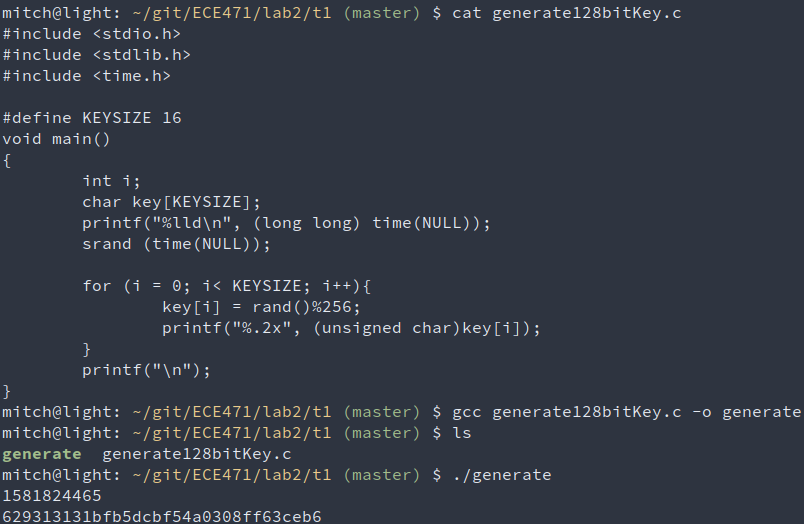
\includegraphics[scale=0.6]{t1p0.png}
    \end{center}{}
    \caption{Compiling and running the generate key program}
    \label{fig:t1p0}
\end{figure}

The output is seemingly random. Let's observe what happens when we run the program multiple times.

\begin{figure}[H]
    \begin{center}
        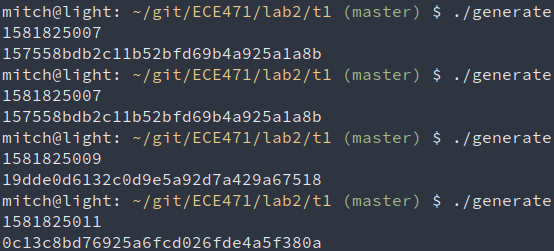
\includegraphics[scale=0.6]{t1p1.png}
    \end{center}{}
    \caption{Running the key generation program multiple times}
    \label{fig:t1p1}
\end{figure}

Figure~\ref{fig:t1p1} shows the output of running the key generation program multiple times. One thing to notice is the first two times that generate is called is that the output is the same. This is because the time command has not refreshed yet. It seems to refresh about every second, which would make a lot of sense. Now lets try it without srand!


\begin{figure}[H]
    \begin{center}
        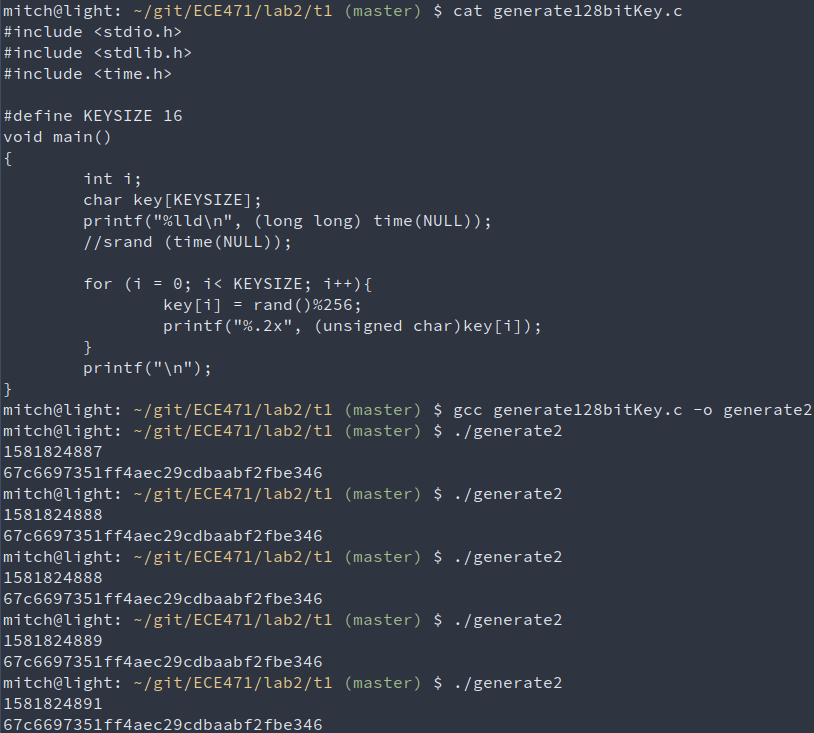
\includegraphics[scale=0.6]{t1p2.png}
    \end{center}{}
    \caption{Running the key generation program without srand multiple times}
    \label{fig:t1p2}
\end{figure}

Figure~\ref{fig:t1p2} shows the result of running the key generation program multiple times. Unline Figure~\ref{fig:t1p1}, the result is always the same. This is because rand has not been randomized with a seed yet.


\subsection{Task 2: Guessing the Key}
On April 17, 2018, Alice finished her tax return, and she saved the return (a PDF file) on her disk. To protect
the file, she encrypted the PDF file using a key generated from the program described in Task 1. She wrote
down the key in a notebook, which is securely stored in a safe. A few month later, Bob broke into her
computer and gets a copy of the encrypted tax return. Since Alice is CEO of a big company, this file is very
valuable.\\
\tab Bob cannot get the encryption key, but by looking around Alice’s computer, he saw the key-generation
program, and suspected that Alice’s encryption key may be generated by the program. He also noticed the
timestamp of the encrypted file, which is "\emph{2018-04-17 23:08:49}". He guessed that the key may be
generated within a two-hour window before the file was created.\\
\tab Since the file is a PDF file, which has a header. The beginning part of the header is always the version
number. Around the time when the file was created, PDF-1.5 was the most common version, i.e., the header
starts with \emph{{\%}PDF-1.5}, which is 8 bytes of data. The next 8 bytes of the data are quite easy to predict as
well. Therefore, Bob easily got the first 16 bytes of the plaintext. Based on the meta data of the encrypted
file, he knows that the file is encrypted using \emph{aes-128-cbc}. Since AES is a 128-bit cipher, the 16-byte
plaintext consists of one block of plaintext, so Bob knows a block of plaintext and its matching ciphertext.
Moreover, Bob also knows the Initial Vector (IV) from the encrypted file (IV is never encrypted). Here is
what Bob knows:
\begin{verbatim}
Plaintext:  255044462d312e350a25d0d4c5d80a34
Ciphertext: d06bf9d0dab8e8ef880660d2af65aa82
IV:         09080706050403020100A2B2C2D2E2F2
\end{verbatim}

\tab Your job is to help Bob find out Alice’s encryption key, so you can decrypt the entire document. You
should write a program to try all the possible keys. If the key was generated correctly, this task will not be
possible. However, since Alice used time() to seed her random number generator, you should be able
to find out her key easily. You can use the date command to print out the number of seconds between a
specified time and the Epoch, 1970-01-01 00:00:00 +0000 (UTC). See the following example.
\begin{verbatim}
$ date -d "2018-04-15 15:00:00" +%s
1523818800
\end{verbatim}

\subsubsection{Task 2: Solution}


We know that the key was generated around 2018-04-17 23:08:49 plus or minus two hours. Therefore, the key was generated between 2018-04-17 21:08:49 and 2018-04-18 1:08:49 The respective seconds between epoch can be found using the date command.

\begin{figure}[H]
    \begin{center}
        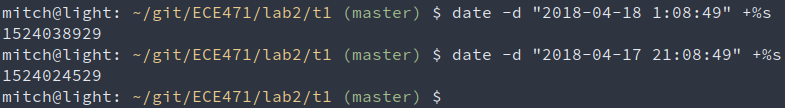
\includegraphics[scale=0.6]{t2p0.png}
    \end{center}{}
    \caption{Finding the window of seconds that the key was generated}
    \label{fig:t2p0}
\end{figure}

Figure~\ref{fig:t2p0} shows that the window of seconds since epoch are between 1524024529 and 1524038929.



K - 
fd89be04ce588454168062267d591d2e

iv -

openssl enc -aes-128-cbc -d -in C -K fd89be04ce588454168062267d591d2e -iv 09080706050403020100A2B2C2D2E2F2

C="d06bf9d0dab8e8ef880660d2af65aa82"
echo "${C}" > C




\clearpage
\subsection{Task 3: Measure the Entropy of Kernel}
In the virtual world, it is difficult to create randomness, i.e., software alone is hard to create random numbers.
Most systems resort to the physical world to gain the randomness. Linux gains the randomness from the
following physical resources:
\begin{verbatim}
void add_keyboard_randomness(unsigned char scancode);
void add_mouse_randomness(__u32 mouse_data);
void add_interrupt_randomness(int irq);
void add_blkdev_randomness(int major);
\end{verbatim}
\tab The first two are quite straightforward to understand: the first one uses the timing between key presses;
the second one uses mouse movement and interrupt timing; the third one gathers random numbers using
the interrupt timing. Of course, not all interrupts are good sources of randomness. For example, the timer
interrupt is not a good choice, because it is predictable. However, disk interrupts are a better measure. The\
last one measures the finishing time of block device requests. \\
\tab The randomness is measured using entropy, which is different from the meaning of entropy in the infor-
mation theory. Here, it simply means how many bits of random numbers the system currently has. You can
find out how much entropy the kernel has at the current moment using the following command.
\begin{verbatim}
$ cat /proc/sys/kernel/random/entropy_avail
\end{verbatim}
\tab Let us monitor the change of the entropy by running the above command via watch, which executes
a program periodically, showing the output in fullscreen. The following command runs the cat program
every 0.1 second.
\begin{verbatim}
$ watch -n .1 cat /proc/sys/kernel/random/entropy_avail
\end{verbatim}
Please run the above command. While it is running, move your mouse, click your mouse, type some-
things, read a large file, visit a website. What activities increases the entropy significantly. Please describe
your observation in your report.

\subsubsection{Task 3: Solution}

The following command is ran:
\begin{verbatim}
$ watch -n .1 cat /proc/sys/kernel/random/entropy_avail
\end{verbatim}

And the results are observed while interacting with the operating system.

\begin{figure}[H]
    \begin{center}
        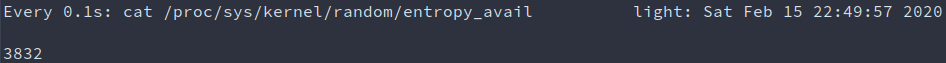
\includegraphics[scale=0.6]{t3p0.png}
    \end{center}{}
    \caption{finding entropy of the system}
    \label{fig:t3p0}
\end{figure}

Figure~\ref{fig:t3p0} shows the entropy when the command is first executed. This shows an entropy of 3832.

\begin{figure}[H]
    \begin{center}
        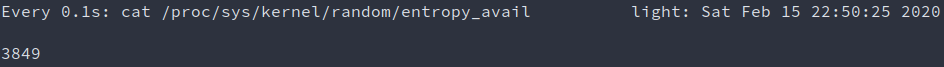
\includegraphics[scale=0.6]{t3p1.png}
    \end{center}{}
    \caption{finding entropy of the system}
    \label{fig:t3p1}
\end{figure}

Figure~\ref{fig:t3p1} shows the entropy after clicking around a little bit. It appears that the entropy is consumed

\begin{figure}[H]
    \begin{center}
        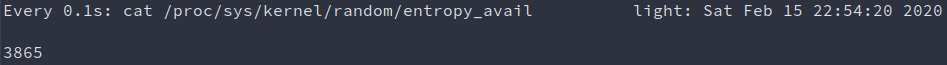
\includegraphics[scale=0.6]{t3p4.png}
    \end{center}{}
    \caption{finding entropy of the system}
    \label{fig:t3p4}
\end{figure}

Figure~\ref{fig:t3p4} shows the entropy after a little bit of web surfing, and creating this lab report. The entropy increases even more! This is likely due to the frequency of my keys, which keys are being pressed, and the coordinates of where my mouse is clicking on the screen. It seems that typing on the keyboard increases the entropy the fastest out of all the sources.

I also decided to do a test where I went to my root directory and had to search for a config file for my Desktop Environment. The following commands were executed:
\begin{verbatim}
cd /
find . -iname "*i3*.conf"
\end{verbatim}
and the entropy gained incredibly fast! Searching the filesystem is awesome for entropy apparently.

\clearpage
\subsection{Task 4: Get Pseudo Random Numbers from /dev/random}
Linux stores the random data collected from the physical resources into a random pool, and then uses
two devices to turn the randomness into pseudo random numbers. These two devices are /dev/random
and /dev/urandom. They have different behaviors. The /dev/random device is a blocking device.
Namely, every time a random number is given out by this device, the entropy of the randomness pool will be
decreased. When the entropy reaches zero, /dev/random will block, until it gains enough randomness. \\
\tab Let us design an experiment to observe the behavior of the /dev/random device. We will use the cat
command to keep reading pseudo random numbers from /dev/random. We pipe the output to hexdump
for nice printing.
\begin{verbatim}
$ cat /dev/random | hexdump
\end{verbatim}
\tab Please run the above command and at the same time use the watch command to monitor the entropy.
What happens if you do not move your mouse or type anything. Then, randomly move your mouse and see
whether you can observe any difference. Please describe and explain your observations.

\textbf{Question}: If a server uses /dev/random to generate the random session key with a client. Please
describe how you can launch a Denial-Of-Service (DOS) attack on such a server.

\subsubsection{Task 4: Solution}


\begin{figure}[H]
    \begin{center}
        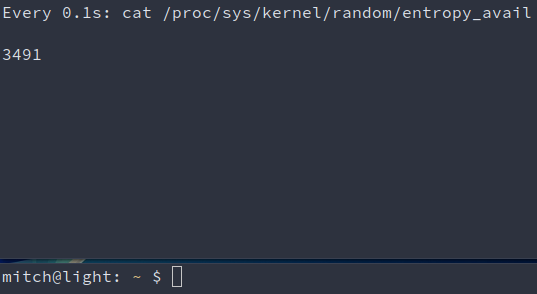
\includegraphics[scale=0.6]{t4p0.png}
    \end{center}{}
    \caption{finding entropy of the system}
    \label{fig:t4p0}
\end{figure}

Figure~\ref{fig:t4p0} shows the entropy of the system before executing the command.

\begin{figure}[H]
    \begin{center}
        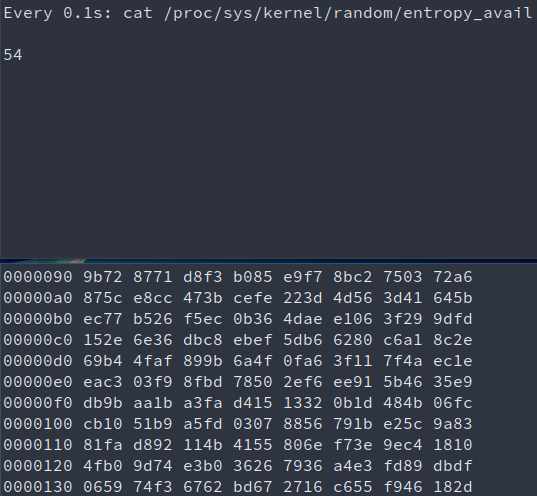
\includegraphics[scale=0.6]{t4p1.png}
    \end{center}{}
    \caption{finding entropy of the system}
    \label{fig:t4p1}
\end{figure}

Figure~\ref{fig:t4p1} shows the entropy after executing the command and waiting for a while. The entropy keeps rising up to 64 and then immediately gets depleted back down to 0. This is because the block size of 64 bytes  that the command uses. The hexdump only produces another line once enough (64 bytes) of entropy is available. The entropy sped up when moving around the mouse rapidly.

\begin{figure}[H]
    \begin{center}
        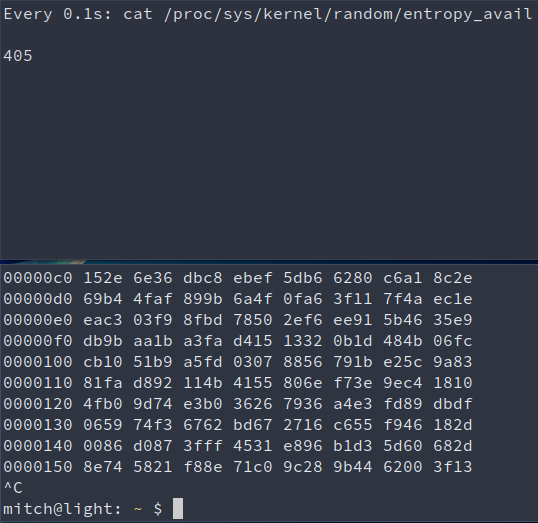
\includegraphics[scale=0.6]{t4p2.png}
    \end{center}{}
    \caption{finding entropy of the system}
    \label{fig:t4p2}
\end{figure}

Figure~\ref{fig:t4p2} shows the entropy after killing the command with a ctr+c command. The entropy is able to finally rise above 64 bytes!

To answer the question at the end, you can execute a DOS attack by simply executing the command cat /dev/random | hexdump with a lot of processes. Since /dev/random is a blocking command, it will halt the execution of other commands if there is not enough bits of entropy.

\clearpage
\subsection{Task 5: Get Random Numbers from /dev/urandom}
Linux provides another way to access the random pool via the /dev/urandom device, except that this
device will not block. Both /dev/random and /dev/urandom use the random data from the pool to
generate pseudo random numbers. When the entropy is not sufficient, /dev/random will pause, while
/dev/urandom will keep generating new numbers. Think of the data in the pool as the “seed”, and as we
know, we can use a seed to generate as many pseudo random numbers as we want. \\
\tab Let us see the behavior of /dev/urandom. We again use cat to get pseudo random numbers from
this device. Please run the following command, and the describe whether moving the mouse has any effect
on the outcome.
\begin{verbatim}
$ cat /dev/urandom | hexdump
\end{verbatim}
\tab Let us measure the quality of the random number. We can use a tool called ent, which has already been
installed in our VM. According to its manual, “ent applies various tests to sequences of bytes stored in files
and reports the results of those tests. The program is useful for evaluating pseudo-random number generators
for encryption and statistical sampling applications, compression algorithms, and other applications where
the information density of a file is of interest”. Let us first generate 1 MB of pseudo random number from
/dev/urandom and save them in a file. Then we run ent on the file. Please describe your outcome, and
analyze whether the quality of the random numbers is good or not.
\begin{verbatim}
$ head -c 1M /dev/urandom > output.bin
$ ent output.bin
\end{verbatim}
\tab Theoretically speaking, the /dev/random device is more secure, but in practice, there is not much
difference, because the “seed” used by /dev/urandom is random and non-predictable (/dev/urandom
does re-seed whenever new random data become available). A big problem of the blocking behavior of
/dev/random is that blocking can lead to denial of service attacks. Therefore, it is recommended that we
use /dev/urandom to get random numbers. To do that in our program, we just need to read directly from
this device file. The following code snippet shows how.
\begin{verbatim}
#define LEN 16
// 128 bits
unsigned char *key = (unsigned char *) malloc(sizeof(unsigned char)*LEN);
FILE* random = fopen("/dev/urandom", "r");
fread(key, sizeof(unsigned char)*LEN, 1, random);
fclose(random);
\end{verbatim}
\tab Please modify the above code snippet to generate a 256-bit encryption key. Please compile and run your
code; print out the numbers and include the screenshot in the report.

\subsubsection{Task 5: Solution}

\begin{figure}[H]
    \begin{center}
        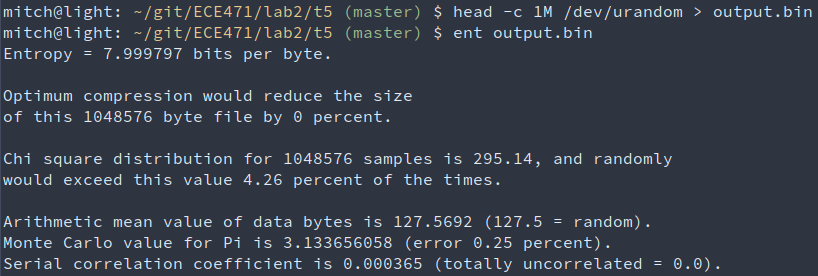
\includegraphics[scale=0.6]{t5p0.png}
    \end{center}{}
    \caption{determining how random /dev/urandom is}
    \label{fig:t5p0}
\end{figure}

Figure~\ref{fig:t5p0} shows the result of executing the code that this task asks to be executed. It appears that the entropy is 7.999797 bits per byte, which is very close an entropy of 1, which is considered completely random. This produced data is very random.

In order to create the 256 bit encryption key, the following script is used:
\begin{verbatim}
#include <stdlib.h>
#include <stdio.h>

#define LEN 32

int main() {
        unsigned char *key = (unsigned char *) malloc(sizeof(unsigned char)*LEN);
        FILE* randomFile = fopen("/dev/urandom", "r");
        fread(key, sizeof(unsigned char)*LEN, 1, randomFile);
        fclose(randomFile);

        printf("%s\n", key);
}
\end{verbatim}

\begin{figure}[H]
    \begin{center}
        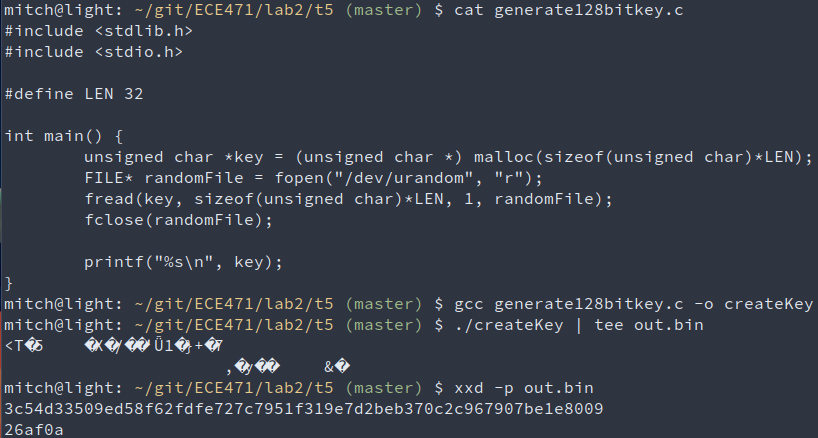
\includegraphics[scale=0.6]{t5p2.png}
    \end{center}{}
    \caption{creating 256 bit encryption key}
    \label{fig:t5p2}
\end{figure}

Figure~\ref{fig:t5p2} shows the results of running the custom script. The data is seemingly random. Let's determine exactly how random is is.

\begin{figure}[H]
    \begin{center}
        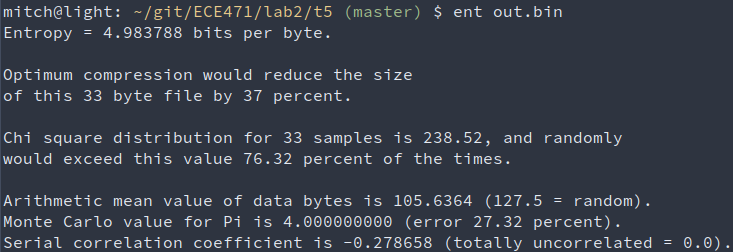
\includegraphics[scale=0.6]{t5p3.png}
    \end{center}{}
    \caption{determining 256 bit random key entropy}
    \label{fig:t5p3}
\end{figure}

Yikes. The entropy of 4.983788 bits per byte is not the best. But it's definitely not the worst!


\end{document}
